\documentclass{report}

\usepackage{../../../../../LaTeX/marzstyle}

\newcommand{\exercisenr}{10}

\runningheads{Network Security}{Exercise \exercisenr}

\setcounter{chapter}{\exercisenr}
\setcounter{section}{3}


\begin{document}
	\section{Question 4}
	\startsection
		\renewcommand{\thesubsection}{\thesection.\Alph{subsection}}
		\subsection{HTTPS operates over three connection levels – HTTP, TLS, and TCP. Have a look at the packet capture in \textit{question4.pcap} and describe, which packets correspond to which of the three levels. Identify the TCP handshake, TLS handshake, HTTP data (specify packet numbers). (Recommendation: use Wireshark)}
		\startsubsection
			\parbox{2.5cm}{\textbf{Packet 1-3}\dotfill} \parbox[t]{12cm}{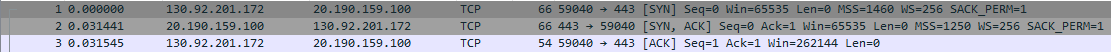
\includegraphics[width=12cm]{packets1-3.png} \\ Port 443 is the standardized port for any HTTPS traffic. Here the connection with the server is established. These three packages are part of the TCP handshake using SYN and ACK packets.} \\
			\parbox{2.5cm}{\textbf{Packet 4}\dotfill} \parbox[t]{12cm}{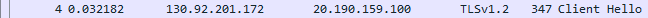
\includegraphics[width=12cm]{packets4.png} \\ Packet 4 is the initialization of the TLS handshake by sending the \textit{Client Hello} message.} \\
			\parbox{2.5cm}{\textbf{Packet 5-9}\dotfill} \parbox[t]{12cm}{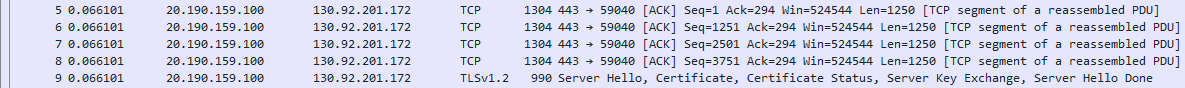
\includegraphics[width=12cm]{packets5-9.png} \\ The marking \textit{[TCP segment of a reassembled PDU]} implies that the packets 5-8 are part of a larger packet. These are used to collect multiple TCP segments for the first stage. Packet 9 contains the \textit{Server Hello}, the certificate, its status, the server key exchange, and the \textit{Server Hello Done}, hence being equivalent to stage 2 from the lecture.} \\
			\parbox{2.5cm}{\textbf{Packet 10}\dotfill} \parbox[t]{12cm}{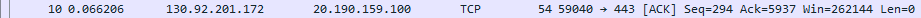
\includegraphics[width=12cm]{packets10.png} \\ The client ackowledges that it received the packet.} \\
			\parbox{2.5cm}{\textbf{Packet 11-17}\dotfill} \parbox[t]{12cm}{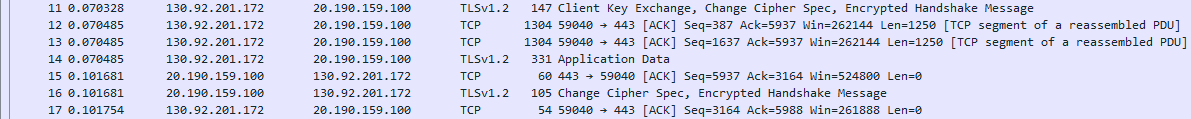
\includegraphics[width=12cm]{packets11-17.png} \\ The cipher suite is changed and in the end the handshake protocol is terminated.} \\
			\parbox{2.5cm}{\textbf{Packet 18-23}\dotfill} \parbox[t]{12cm}{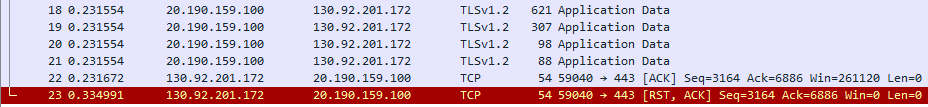
\includegraphics[width=12cm]{packets18-23.png} \\ In these packets HTTP data is sent which is said to be any \textit{Application Data}.} \\ \\
			With these information we can say that packet 4 until packet 17 is the TLS handshake.
		\closesection
		\subsection{Is mutual authentication in place in the TLS handshake from question 4 A?}
		\startsubsection
			\parbox{2cm}{\textbf{Phase 2}\dotfill} \parbox[t]{12.5cm}{As the server sends its own certificate it is obviously authenticated. However, it is particular that no \textit{certificate\_request message} was sent which requests a certificate from the client.} \\
			\\\parbox{2cm}{\textbf{Phase 3}\dotfill} \parbox[t]{12.5cm}{As a baseline the book \textit{Cryptography and Network Security Principles and Practice Seventh Edition page 560} is used: The server starts phase 3 by requesting a certificate from the client. As described above this is what is happening so both sides are authenticated to each other. However, it is ver particular that no \textit{certificate\_verify} message is sent in order to verify the certificates.} \\
		\closesection
	\closesection
\end{document}